% Rozdział 24 – Szachownice, klocki i kolorowanie

\theory{Szachownice, klocki i kolorowanie}

\noindent
Zajmiemy się teraz zadaniami związanymi z planszami, wypełnianiem ich klockami oraz dowodzeniem, że to nie jest możliwe. Bardzo często wykonuje się to za pomocą pokolorowania lub wpisania odpowiednich liczb w pola planszy.

\vspace{10px}

\heading{Przykład 1}

\noindent
Szachownicę o wymiarach $2018\times 2018$ przykryto przy pomocy jednej kwadratowej płytki o wymiarach $2 \times 2$ oraz $\frac{2018^2 − 4}{5}$ prostokątnych płytek o wymiarach $1 \times 5$ w taki sposób, że każde pole szachownicy jest przykryte przez dokładnie jedną płytkę (płytki można obracać). Wykazać, że płytka 2 × 2 nie przykrywa żadnego pola o krawędzi zawartej w brzegu szachownicy.

\vspace{5px}

\heading{Rozwiązanie}

\noindent
Wpiszmy w pola planszy liczby, tak jak to zrobiono na rysunku. W pierwszym wierszu są liczby $1$, w drugim liczby $2$, ..., w piątym liczby $5$, w szóstym znowu $1$, w siódmym dwa itd. Innymi słowy w każde pole wpisujemy resztę z dzielenia numeru wiersza przez $5$.

\begin{center}
	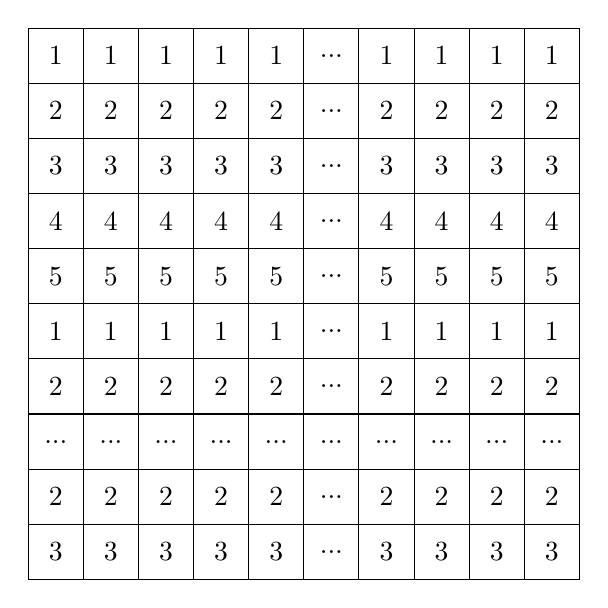
\begin{tikzpicture}[scale=0.7]
		\draw (0,0) -- (10,0) -- (10,10) -- (0,10) -- cycle;
		\draw (0,1) -- (10,1);
		\draw (0,2) -- (10,2);
		\draw (0,3) -- (10,3);
		\draw (0,4) -- (10,4);
		\draw (0,5) -- (10,5);
		\draw (0,6) -- (10,6);
		\draw (0,7) -- (10,7);
		\draw (0,8) -- (10,8);
		\draw (0,9) -- (10,9);


		\draw (1,0) -- (1,10);
		\draw (2,0) -- (2,10);
		\draw (3,0) -- (3,10);
		\draw (4,0) -- (4,10);
		\draw (5,0) -- (5,10);
		\draw (6,0) -- (6,10);
		\draw (7,0) -- (7,10);
		\draw (8,0) -- (8,10);
		\draw (9,0) -- (9,10);
		\draw (10,0) -- (10,10);

		\node at (0.5,9.5) {1};
		\node at (1.5,9.5) {1};
		\node at (2.5,9.5) {1};
		\node at (3.5,9.5) {1};
		\node at (4.5,9.5) {1};
		\node at (5.5,9.5) {...};
		\node at (6.5,9.5) {1};
		\node at (7.5,9.5) {1};
		\node at (8.5,9.5) {1};
		\node at (9.5,9.5) {1};

		\node at (0.5,8.5) {2};
		\node at (1.5,8.5) {2};
		\node at (2.5,8.5) {2};
		\node at (3.5,8.5) {2};
		\node at (4.5,8.5) {2};
		\node at (5.5,8.5) {...};
		\node at (6.5,8.5) {2};
		\node at (7.5,8.5) {2};
		\node at (8.5,8.5) {2};
		\node at (9.5,8.5) {2};

		\node at (0.5,7.5) {3};
		\node at (1.5,7.5) {3};
		\node at (2.5,7.5) {3};
		\node at (3.5,7.5) {3};
		\node at (4.5,7.5) {3};
		\node at (5.5,7.5) {...};
		\node at (6.5,7.5) {3};
		\node at (7.5,7.5) {3};
		\node at (8.5,7.5) {3};
		\node at (9.5,7.5) {3};

		\node at (0.5,6.5) {4};
		\node at (1.5,6.5) {4};
		\node at (2.5,6.5) {4};
		\node at (3.5,6.5) {4};
		\node at (4.5,6.5) {4};
		\node at (5.5,6.5) {...};
		\node at (6.5,6.5) {4};
		\node at (7.5,6.5) {4};
		\node at (8.5,6.5) {4};
		\node at (9.5,6.5) {4};

		\node at (0.5,5.5) {5};
		\node at (1.5,5.5) {5};
		\node at (2.5,5.5) {5};
		\node at (3.5,5.5) {5};
		\node at (4.5,5.5) {5};
		\node at (5.5,5.5) {...};
		\node at (6.5,5.5) {5};
		\node at (7.5,5.5) {5};
		\node at (8.5,5.5) {5};
		\node at (9.5,5.5) {5};

		\node at (0.5,4.5) {1};
		\node at (1.5,4.5) {1};
		\node at (2.5,4.5) {1};
		\node at (3.5,4.5) {1};
		\node at (4.5,4.5) {1};
		\node at (5.5,4.5) {...};
		\node at (6.5,4.5) {1};
		\node at (7.5,4.5) {1};
		\node at (8.5,4.5) {1};
		\node at (9.5,4.5) {1};

		\node at (0.5,3.5) {2};
		\node at (1.5,3.5) {2};
		\node at (2.5,3.5) {2};
		\node at (3.5,3.5) {2};
		\node at (4.5,3.5) {2};
		\node at (5.5,3.5) {...};
		\node at (6.5,3.5) {2};
		\node at (7.5,3.5) {2};
		\node at (8.5,3.5) {2};
		\node at (9.5,3.5) {2};



		\node at (0.5,2.5) {...};
		\node at (1.5,2.5) {...};
		\node at (2.5,2.5) {...};
		\node at (3.5,2.5) {...};
		\node at (4.5,2.5) {...};
		\node at (5.5,2.5) {...};
		\node at (6.5,2.5) {...};
		\node at (7.5,2.5) {...};
		\node at (8.5,2.5) {...};
		\node at (9.5,2.5) {...};


		\node at (0.5,1.5) {2};
		\node at (1.5,1.5) {2};
		\node at (2.5,1.5) {2};
		\node at (3.5,1.5) {2};
		\node at (4.5,1.5) {2};
		\node at (5.5,1.5) {...};
		\node at (6.5,1.5) {2};
		\node at (7.5,1.5) {2};
		\node at (8.5,1.5) {2};
		\node at (9.5,1.5) {2};


		\node at (0.5,0.5) {3};
		\node at (1.5,0.5) {3};
		\node at (2.5,0.5) {3};
		\node at (3.5,0.5) {3};
		\node at (4.5,0.5) {3};
		\node at (5.5,0.5) {...};
		\node at (6.5,0.5) {3};
		\node at (7.5,0.5) {3};
		\node at (8.5,0.5) {3};
		\node at (9.5,0.5) {3};
	\end{tikzpicture}
\end{center}

\noindent
Zauważmy, że suma liczb pokrytych klocek $1 \times 5$ zawsze będzie podzielna przez $5$. W tablicy jest po $403$ rzędów zawierających same czwórki lub same piątki oraz $404$ rzędów zawierających same jedynki, same dwójki lub same trójki. Suma wszystkich liczb zapisanych w tablicy wynosi więc
\[
	2018( 1 \cdot 404 + 2\cdot 404 + 3 \cdot 404 + 4 \cdot 403 + 5 \cdot 403) \equiv 3 \pmod{5}.
\] 
Stąd płytka $2\times2$ musi pokrywać liczby o sumie dającej resztę $3$ z dzielenia przez $5$. Jeśli leżałaby przy górnej krawędzi planszy, to dawałaby resztę
\[
	1 + 1 + 2 + 2 \equiv 1 \pmod{5},
\]
czyli nie może tam się znajdować. Analogicznie pokazujemy, że płytka $2 \times 2$ nie leży przy żadnej z pozostałych krawędzi.

\qed

\noindent
Rozwiązując zadania podobne do powyższego zawsze warto rozważyć jak najwięcej możliwych kolorowań/wpisań liczb i zobaczyć, czy z któregoś z nich coś wynika. Nie ma tutaj przepisu, który zawsze działa -- trzeba robić to metodą prób i błędów. Warto zwrócić szczególną uwagę na takie kolorowania, że rozpatrywana płytka zawsze pokrywa tę samą liczbę pokolorowanych pól lub suma liczb pokrytych przez klocek zawsze ma pewną właściwość.

\vspace{10px}
\noindent
Teraz kolej na przykład pięknego, choć trudnego, zadania z teorii grafów z bardzo ciekawym zastosowaniem kolorowań.

\vspace{10px}

\heading{Przykład 2}

\noindent
Dany jest graf. W każdym ruchu na aktualnym grafie $G$ można wykonać jedną z dwóch operacji

\begin{itemize}

\item Jeśli pewien wierzchołek ma nieparzysty stopień, to usunąć wszystkie krawędzie, które z niego wychodzą.


\item Można dodać do grafu $G$ graf $G'$ będący kopią grafu $G$. Następnie łączymy odpowiadające sobie wierzchołki z $G$ oraz $G'$. 
\end{itemize}

\noindent
Wykazać, że niezależnie od grafu początkowego, można wykonać pewną liczbę operacji, aby otrzymać graf bez żadnej krawędzi.

\vspace{5px}


\begin{center}
	\begin{tikzpicture}
		\tikzset{vertex/.style = {shape=circle,draw, inner sep = 1pt, fill=black}}

		\node[vertex] (A_1) at (1,2) {};
		\node[vertex] (A_2) at (0,1) {};
		\node[vertex] (A_4) at (1,-1) {};




		\draw (A_1)--(A_2);

	\end{tikzpicture}
	\begin{tikzpicture}
		\tikzset{vertex/.style = {shape=circle,draw, inner sep = 1pt, fill=black}}

		\node[vertex] (A_1) at (1,2) {};
		\node[vertex] (A_2) at (0,1) {};
		\node[vertex, label=left:$X$] (A_3) at (0,0) {};
		\node[vertex] (A_4) at (1,-1) {};




		\draw (A_1)--(A_2);
		\draw (A_2)--(A_3);
		\draw (A_3)--(A_4);
		\draw (A_1)--(A_3);

		%arrows


		\draw (-1,0.5) -- (-2,0.5);
		\draw (-1.7,0.2) -- (-2,0.5);
		\draw (-1.7,0.7) -- (-2,0.5);

	\end{tikzpicture}	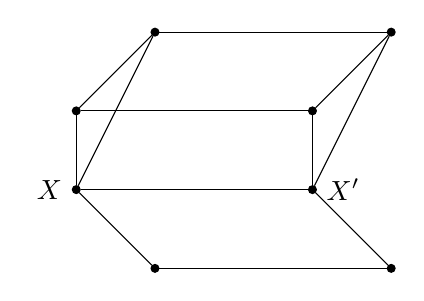
\begin{tikzpicture}
		\tikzset{vertex/.style = {shape=circle,draw, inner sep = 1pt, fill=black}}

		\node[vertex] (A_1) at (1,2) {};
		\node[vertex] (A_2) at (0,1) {};
		\node[vertex, label=left:$X$] (A_3) at (0,0) {};
		\node[vertex] (A_4) at (1,-1) {};

		\node[vertex] (B_1) at (4,2) {};
		\node[vertex] (B_2) at (3,1) {};
		\node[vertex, label=right:$X'$] (B_3) at (3,0) {};
		\node[vertex] (B_4) at (4,-1) {};




		\draw (A_1)--(A_2);
		\draw (A_2)--(A_3);
		\draw (A_3)--(A_4);
		\draw (A_1)--(A_3);

		\draw (B_1)--(B_2);
		\draw (B_2)--(B_3);
		\draw (B_3)--(B_4);
		\draw (B_1)--(B_3);



		\draw (A_1)--(B_1);
		\draw (A_2)--(B_2);
		\draw (A_3)--(B_3);
		\draw (A_4)--(B_4);

	\end{tikzpicture}\\
	\noindent
	W powyższym przykładzie możemy chociażby usunąć wierzchołek $X$, albo wykonać dodać do grafu jego kopię.
\end{center}

\heading{Rozwiązanie}

\noindent
Pokolorujmy każdy z wierzchołków grafu $G$, tak, aby żadne dwa wierzchołki połączone krawędzią nie były tego samego koloru.
Niech $\chi(G)$ oznacza minimalną liczbę kolorów, dla których takie kolorowanie istnieje. Liczbę $\chi(G)$ będziemy nazywać \textit{liczbą chromatyczną} grafu $G$.

\vspace{10px}
\noindent
Wykażemy, że jeśli graf $G$ zawiera pewną krawędź, to zawsze istnieje ciąg ruchów, który zmniejszy liczbę chromatyczną danego grafu $G$. Jeśli ta liczba wyniesie $1$, to będzie oznaczało, że nie $G$ nie zawiera już żadnej krawędzi. Stąd też wyniknie teza.

\vspace{10px}
\noindent
Najpierw usuniemy wszyskie wierzchołki, które możemy usunąć. Oczywiście ta operacja nie zwiększy liczby chromatycznej. Otrzymamy w ten sposób graf $G$, w którym nie da się usunąć żadnego wierzchołka -- wszystkie one mają parzysty stopień.

\begin{center}
	\begin{tikzpicture}
		\tikzset{vertex/.style = {shape=circle,draw, inner sep = 1pt, fill=black}}

		\node[vertex, label=above:$0$] (A_1) at (1,2) {};
		\node[vertex, label=left:$1$] (A_2) at (0,1) {};
		\node[vertex, label=left:$0$] (A_3) at (0,0) {};
		\node[vertex, label=below:$1$] (A_4) at (1,-1) {};


		\draw (2,0.5) -- (3,0.5);
		\draw (2.7,0.2) -- (3,0.5);
		\draw (2.7,0.7) -- (3,0.5);


		\draw (A_1)--(A_2);
		\draw (A_2)--(A_3);
		\draw (A_3)--(A_4);
		\draw (A_1)--(A_4);

	\end{tikzpicture}
	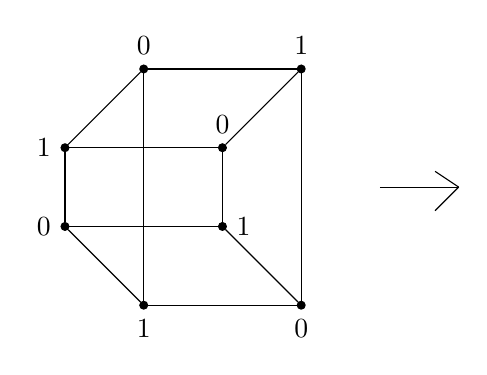
\begin{tikzpicture}
		\tikzset{vertex/.style = {shape=circle,draw, inner sep = 1pt, fill=black}}

		\node[vertex, label=above:$0$] (A_1) at (1,2) {};
		\node[vertex, label=left:$1$] (A_2) at (0,1) {};
		\node[vertex, label=left:$0$] (A_3) at (0,0) {};
		\node[vertex, label=below:$1$] (A_4) at (1,-1) {};

		\draw (A_1)--(A_2);
		\draw (A_2)--(A_3);
		\draw (A_3)--(A_4);
		\draw (A_1)--(A_4);

		\node[vertex, label=above:$1$] (B_1) at (3,2) {};
		\node[vertex, label=above:$0$] (B_2) at (2,1) {};
		\node[vertex, label=right:$1$] (B_3) at (2,0) {};
		\node[vertex, label=below:$0$] (B_4) at (3,-1) {};

		\draw (B_1)--(B_2);
		\draw (B_2)--(B_3);
		\draw (B_3)--(B_4);
		\draw (B_1)--(B_4);

		\draw (A_1)--(B_1);
		\draw (A_2)--(B_2);
		\draw (A_3)--(B_3);
		\draw (A_4)--(B_4);


		\draw (4,0.5) -- (5,0.5);
		\draw (4.7,0.2) -- (5,0.5);
		\draw (4.7,0.7) -- (5,0.5);

	\end{tikzpicture}
	\begin{tikzpicture}
		\tikzset{vertex/.style = {shape=circle,draw, inner sep = 1pt, fill=black}}

		\node[vertex, label=above:$0$] (A_1) at (1,2) {};
		\node[vertex, label=left:$0$] (A_3) at (0,0) {};


		\node[vertex, label=above:$0$] (B_2) at (2,1) {};
		\node[vertex, label=below:$0$] (B_4) at (3,-1) {};

	\end{tikzpicture}
\end{center}

\vspace{10px}
\noindent
Następnie użyjmy operacji drugiego typu -- połączmy graf $G$ z jego kopią. Najpierw wykażemy, że liczba chromatyczna otrzymanego grafu jest nie większa niż liczba chromatyczna grafu $G$. Załóżmy, że wierzchołki grafu $G$ da się pokolorować kolorami o numerach od $0$ do $\chi(G) - 1$, gdzie $\chi(G) \geqslant 2$ (w przeciwnym wypadku łatwo uzyskujemy tezę). Pokolorujmy $G'$ w następujący sposób: 
Jeśli wierzchołek $X \in G$ ma kolor $k$, to odpowiadający mu wierzchołek $X' \in G'$ ma pokolorujemy na kolor o numerze $k + 1 \text{ mod } \chi(G)$. Łatwo sprawdzić, że takie kolorowanie spełnia warunki zadania.

\vspace{10px}
\noindent
Przed poprzednią operacją każdy wierzchołek miał stopień parzysty, a więc po jej wykonaniu każdy z wierzchołków będzie miał stopień nieparzysty. Wybierzmy jeden z kolorów -- możemy za pomocą pierwszej operacji usunąć wszystkie wierzchołki tego koloru. Istotnie, żadne dwa nie sąsiadują ze sobą, więc usunięcie jednego z nich nie wywrze wpływu na stopień innego wierzchołka tego samego koloru. Po usunięciu wszystkich wierzchołków jednego koloru otrzymamy graf, który jest pokolorowany co najwyżej $\chi(G) - 1$ kolorami. Ma więc on mniejszą liczbę chromatyczną niż graf $G$, czego należało dowieść.

\qed

\noindent
Powyższe rozwiązanie jest bardzo pomysłowe. Czytelniczkę/czytelnika może zastanawiać jak na nie wpaść. Nie ma tutaj sposobu ze $100\%$ skutecznością, ale pewne rzeczy mogą pomóc. Przede wszystkim warto próbować jak największej liczby pomysłów. Nawet tych, które na pierwszy rzut oka nie mają wielkiego sensu. Równie ważna jest umiejętność szybkiego rozpoznania, że dany pomysł nie może doprowadzić do rozwiązania. Poza tym niektóre pomysły po prostu trzeba znać, a taka znajomość może zostać wyrobiona jedynie przez rozwiązywanie zadań.

\vspace{10px}
\begin{remark}
W każdym z poniższych zadań zakładamy, że klocki, którymi wypełniamy szachownice można obracać.
\end{remark}
\vspace{5px}
